\documentclass[12pt]{article}
\usepackage[utf8]{inputenc}
\newcommand\preamble{
    \usepackage[italian]{babel}
    \usepackage{geometry}
    \usepackage{amsmath}
    \usepackage{amssymb}
    \usepackage{graphicx}
    \usepackage{ulem}
    \usepackage[dvipsnames]{xcolor}

    \geometry{margin=2cm}
    \let\olditemize\itemize
    \renewcommand\itemize{\olditemize\setlength\itemsep{0em}}
    \graphicspath{{../Immagini/}}

    \author{Lorenzo Vaccarecci}
}
\preamble

\title{Progettazione Logica e Inverse Engineering}
\date{19 Marzo 2024}

\begin{document}
\maketitle
\section{Ristrutturazione (continuazione)}
\subsection{Analisi delle ridondanze}
\begin{center}
    \begin{tikzpicture}[auto, node distance=3.5cm]
        \node[entity] (studente) {Studente}
        child[grow=left,level distance=3cm] {node[attribute] (cfu){cfu acquisiti}}
        child[grow=up] {node[attribute] (media){media}}
        child[grow=down] {node[attribute] (matricola){\key{matricola}}};
        ;
        \node[relationship] (registrazione) [right of=studente] {reg carr}
        child {node[attribute] (voto){voto}}
        child {node[attribute] (data){data}}
        ;
        \node[entity] (insegnamento) [right of=registrazione] {Insegnamento}
        child {node[attribute] (codice) {\key{Codice}}}
        ;
        \draw (studente) -- node{($0$,$n$)} (registrazione);
        \draw (registrazione) -- node{($0$,$n$)} (insegnamento);
    \end{tikzpicture}
\end{center}
In questo caso è ridondante la presenza dell'attributo \textit{media} in quanto può essere ricavata usando \textit{voto}.
Un altro caso è quando abbiamo un'associazione "inutile" come ad esempio:
\begin{center}
    \begin{tikzpicture}[auto, node distance=2.5cm]
        \node[entity] (film) {Film};
        \node[relationship] (in) [right of=film] {in};
        \node[relationship] (nel di) [below right of=film] {nel di};
        \node[entity] (video)[right of=in] {Video};
        \node[relationship] (di) [below of=video] {di};
        \node[entity] (noleggio)[below of=di] {Noleggio};
        \draw (film) -- node{} (in);
        \draw (film) -- node{} (nel di);
        \draw (video) -- node{} (in);
        \draw (video) -- node{} (di);
        \draw (noleggio) -- node{$(1,1)$} (nel di);
        \draw (noleggio) -- node{$(1,1)$} (di);
    \end{tikzpicture}
\end{center}
\begin{description}
    \item[Partizionamento Orizzontale]: alcune righe di una tabella vengono spostate in una nuova tabella
    \item[Partizionamento Verticale]: alcune colonne di una tabella vengono spostate in una nuova tabella
\end{description}
\section{Traduzione}
Una entità diventerà una relazione:
\begin{center}
    \begin{tikzpicture}[auto, node distance=2.5cm]
        \node[entity] (e) {E}
        child {node[attribute] (k) {\key{k}}}
        child {node[attribute] (a1) {A1}}
        child {node[attribute] (a2) {A2}};
        ;
        \node [below of= e]{\large E(\key{k}, A1, A2)};
    \end{tikzpicture}
\end{center}
Nel caso delle chiavi esterne:
\begin{center}
    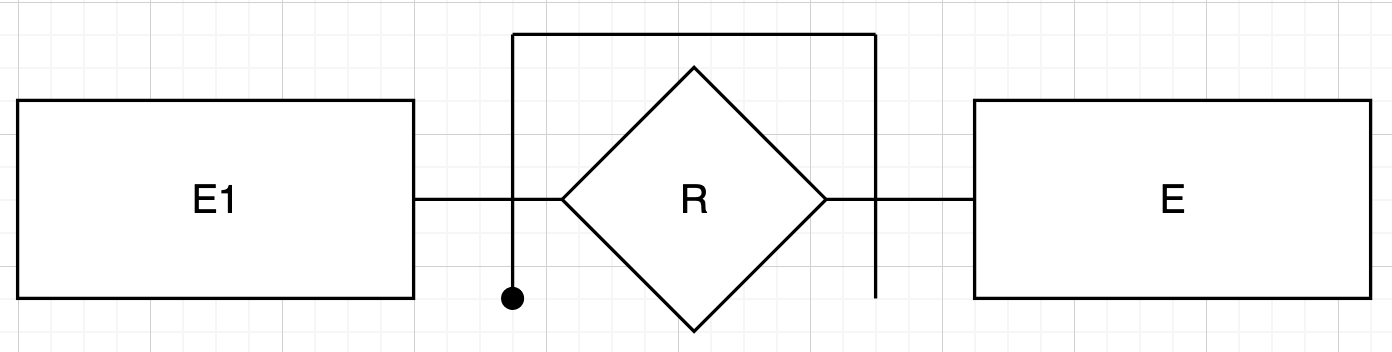
\includegraphics[width=\textwidth]{chiaveesterna.png}
\end{center}
E(\key{k}, A1, A2)\\
E1(\key{k$^{E}$}, A3, A4)\\
\end{document}